%===================================== CHAP 5 =================================

\chapter{Experimental testing}
This chapter contain the result from the test that were performed. The goal with these tests was to test the performance of the Ublox LEA M8T, compare the performance of \acrfull{rtklib} with Piksi, and to compare the real time estimate from both system with the post-processed solution. The comparison test was performed with the pixi and ublox connected to the same antenna at both the rover and the base station. Then the deviation in the position estimate can only come from the receivers. All position and velocity data is given in the \gls{ned} frame, however altitude is used for the flight test.
\section{Performance testing of UAV Position System}
The experimental test was split in two independent test, one where the X8 \gls{uav} was carried around on a open field to test the performance of the \gls{rtk-gps} system in a more controlled environment. The goal of the first was to log data from both \gls{rtk-gps} system in optimal condition for the navigation system. The second test was perform in a more realistic environment for a navigation system. 


\subsection{Test 1: Test of the RTK-GPS navigation system}
In this part two test of navigation data will be presented. Both tests were performed on the same day, which was cloudless and at a time with low \gls{dop}. The raw data from the Ublox receiver was post processed with rtklib, and it should be more accurate than its real time counter part. Therefore a estimate of error was defined as:
\begin{equation}
e(t) = p_r(t) - p_p(t)
\end{equation}
where $p_r(t)$ and $p_p(t)$ is defined as the position solution from the real time system and the position solution from the post processed solution respectfully. $e(t)$ is used as a measure on the performance of the position estimate relative to the assumed more accurate post-processed estimate. It should be noted that in order to compare the different time-series the position data was synchronized with each other. From the error the cumulative standard deviation was calculated using the matlab function "std".
\subsubsection{First test}
In the first session of the test the \gls{uav} was carried around on a open field, and latter placed exactly on the same place where it started. As expected both systems provided a position estimate with fixed integer solution that followed the true path, and further confirms that both system performed in a similar manner. Therefore both systems are suitable for further comparison of position estimation in a flying test.
Figure \ref{figure:xywalk1} shows a North East plot of how the walk was. The plot contain only the fixed solution from both the piksi and rtklib. 
\begin{figure}[H]
	\centering
		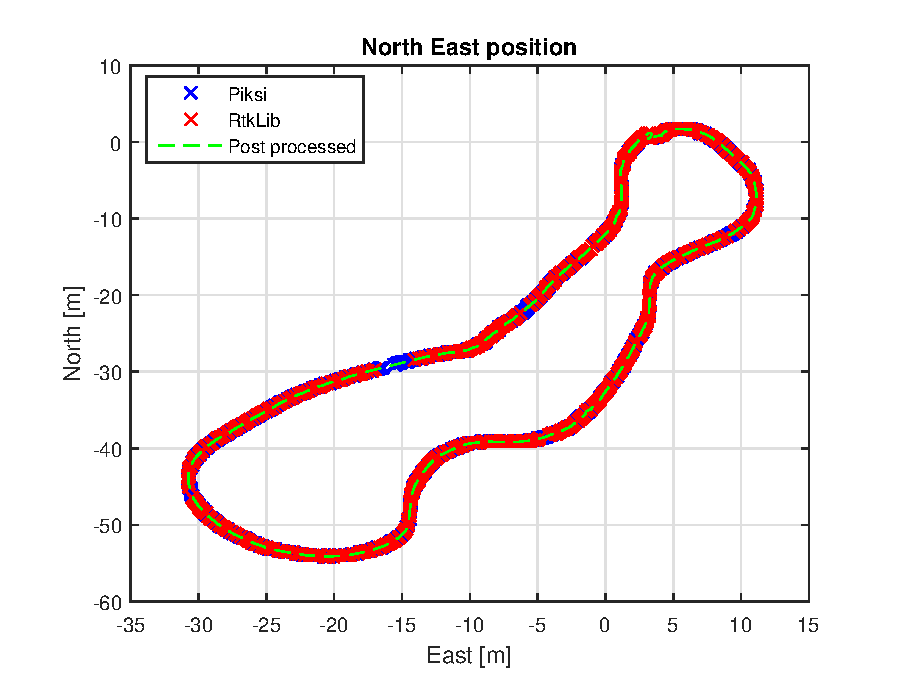
\includegraphics[width=0.7\textwidth]{figs/plots/xywalk1.eps}
		\caption{A xy plot of the piksi,rtklib real time solution and the rtklib post processed solution}
		\label{figure:xywalk1}
\end{figure}
Figure \ref{figure:DownAndAmbwalk1} shows the down position, as well as how the integer ambiguity solution was during the experiment. As seen in the figure both the Piksi and Rtklib manage to keep there fixed solution. The position solution from both the Piksi and Rtklib agrees with the post processed solution. 
\begin{figure}[H]
	\centering
		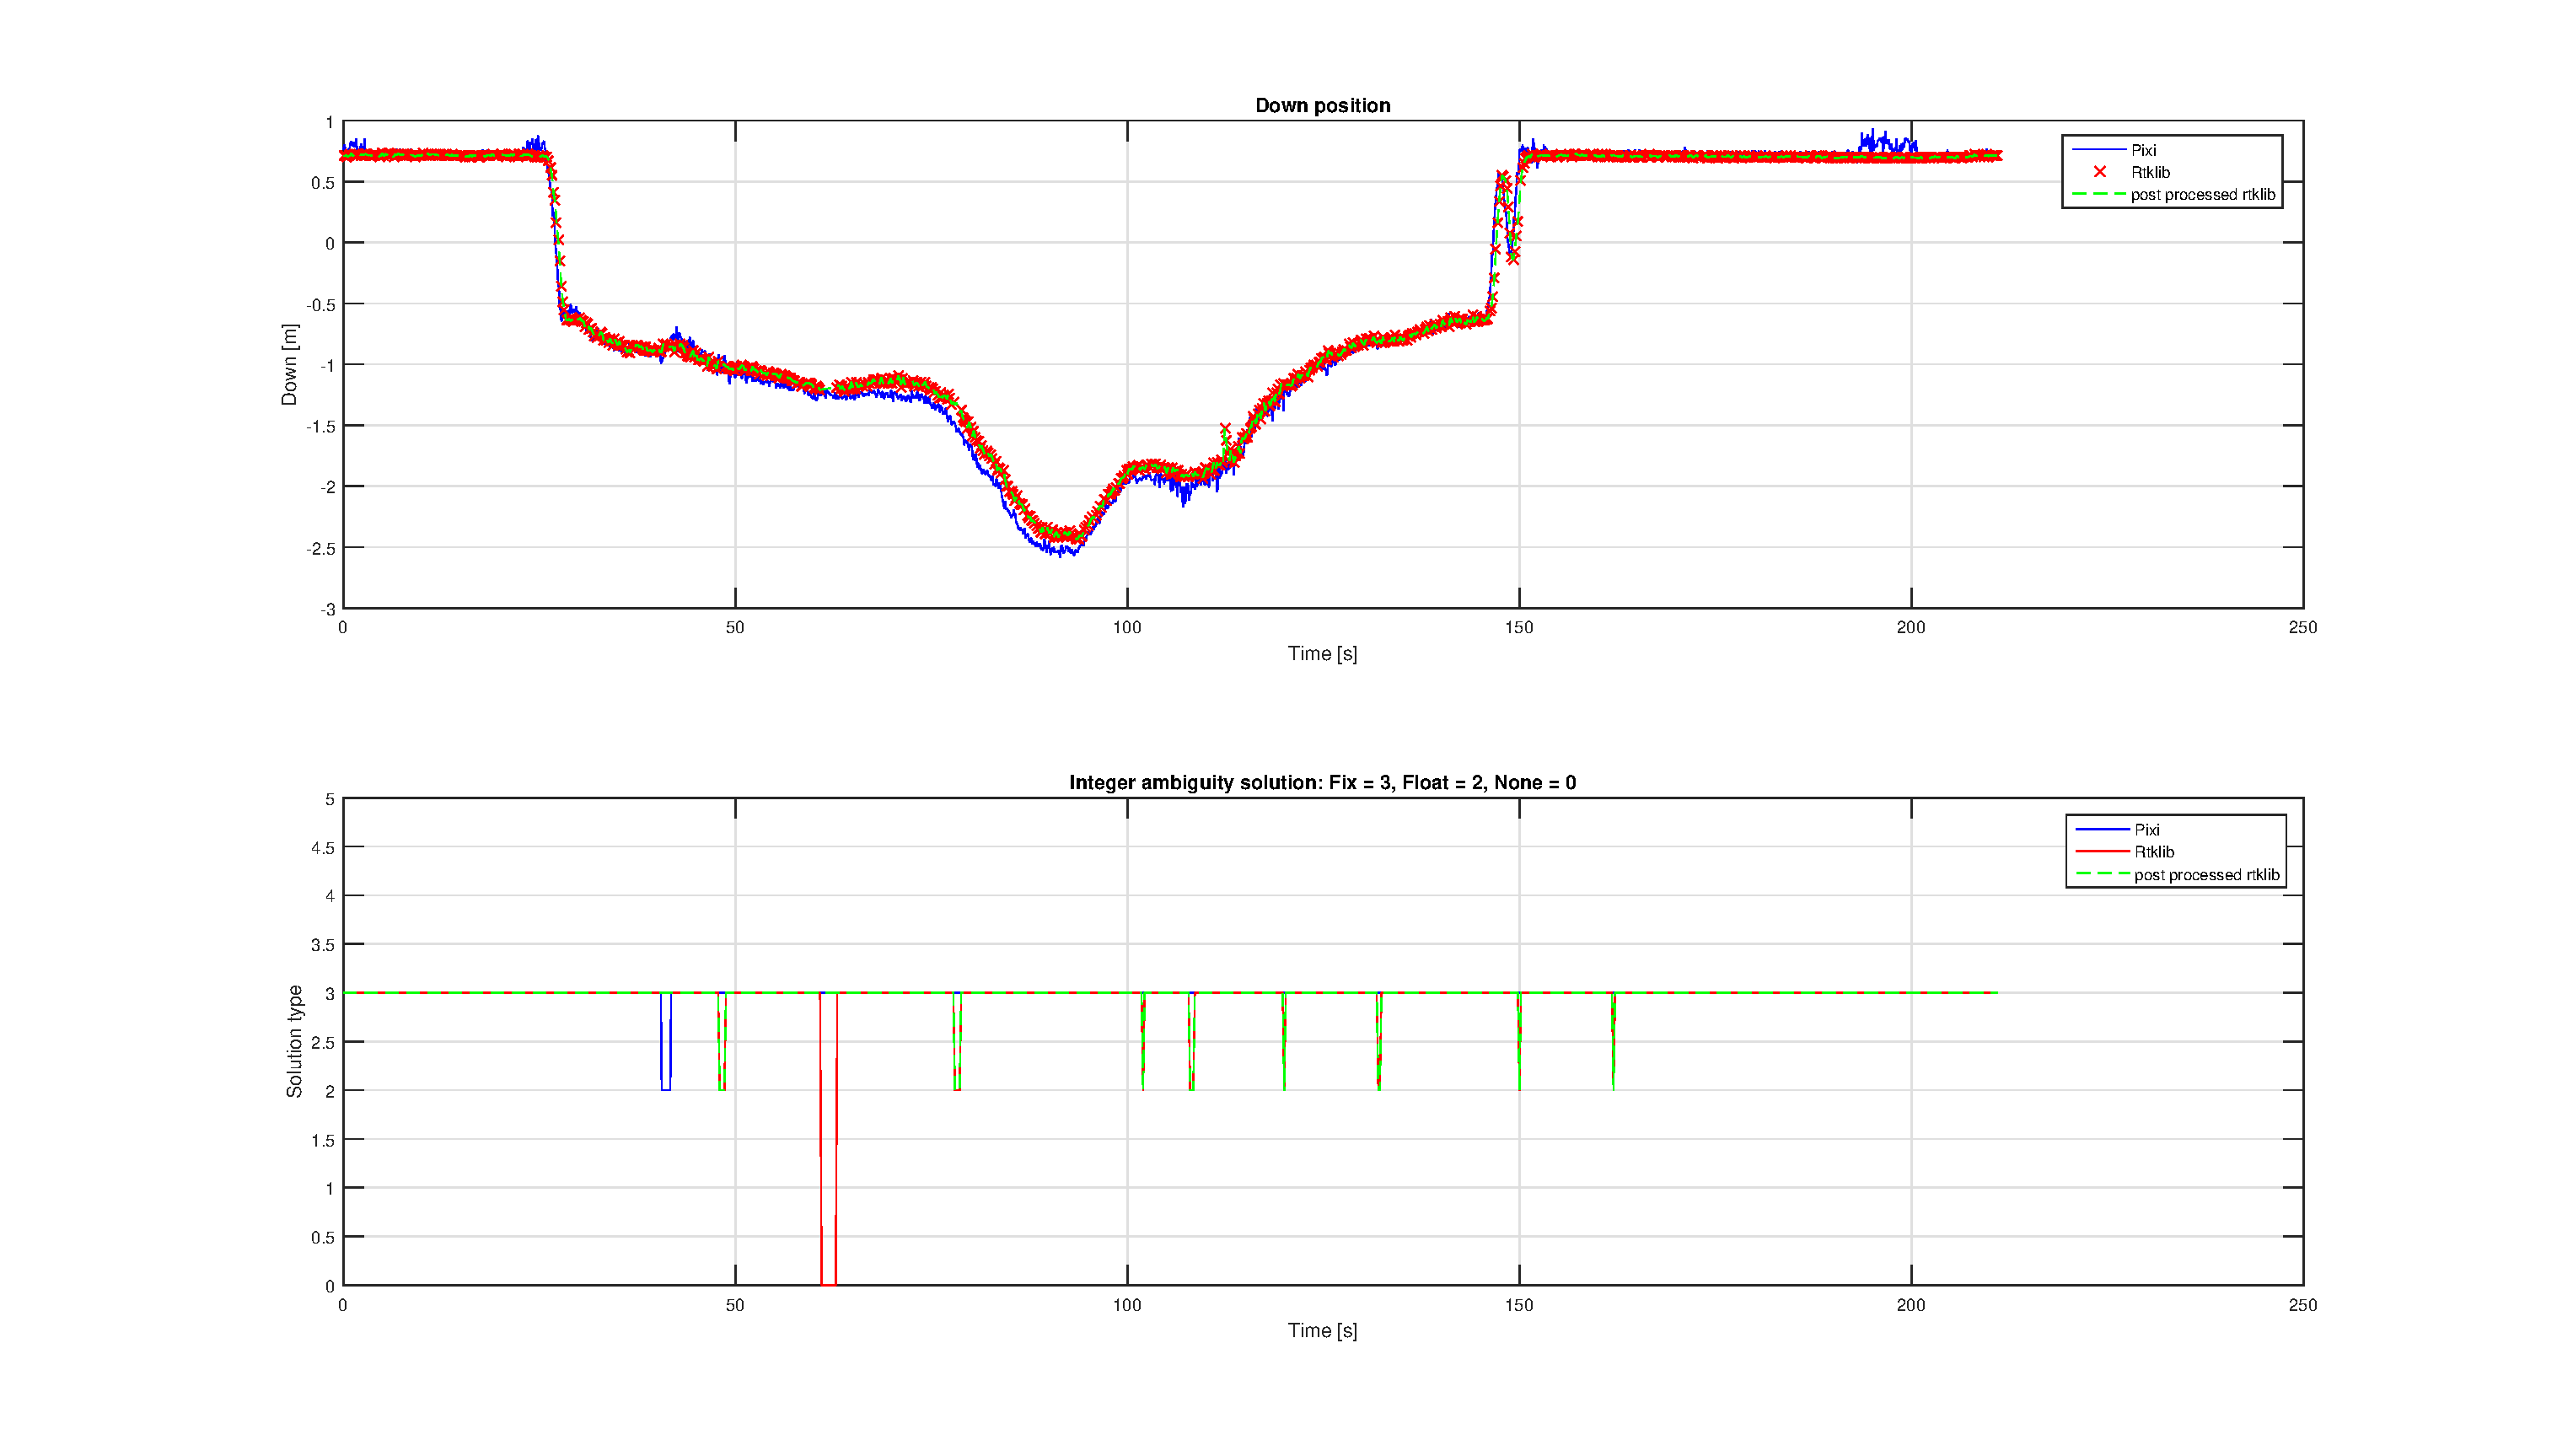
\includegraphics[width=0.7\textwidth]{figs/plots/downWalk1.eps}
		\caption{The communication structure of rtklib}
		\label{figure:DownAndAmbwalk1}
\end{figure}

As seen in figure \ref{figure:xywalk1} the difference between the different solution is quite small, which is confirmed in the error plot shown in figure \ref{figure:errorRTKwalk1} and \ref{figure:errorPiksiwalk1}
\begin{figure}[H]
	\centering
		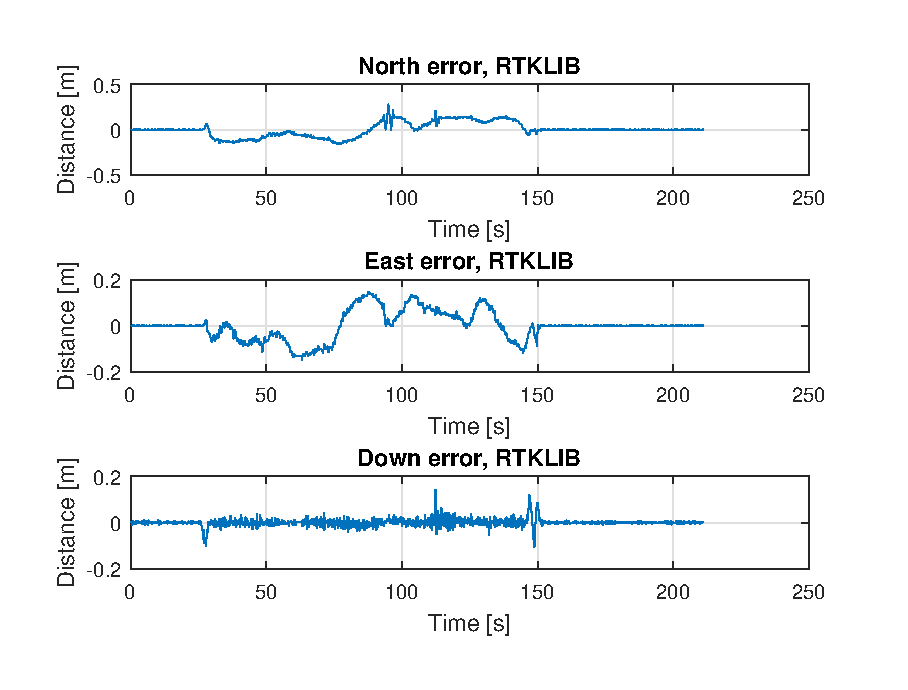
\includegraphics[width=0.7\textwidth]{figs/plots/errorRtklibWalk1.eps}
		\caption{The difference between rtklib real time and post processed solution}
		\label{figure:errorRTKwalk1}
\end{figure}
\begin{figure}[H]
	\centering
		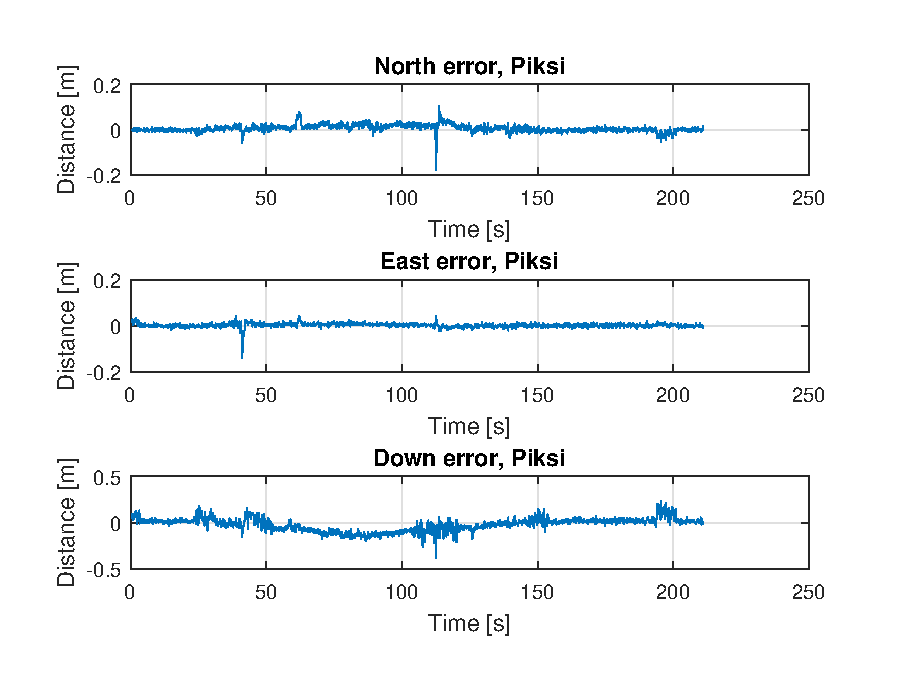
\includegraphics[width=0.7\textwidth]{figs/plots/errorPiksiWalk1.eps}
		\caption{The communication structure of rtklib}
		\label{figure:errorPiksiwalk1}
\end{figure}
The cumulative standard deviation for the error from both the Piksi and \gls{rtklib} indicate that the estimate has a high precision, as seen in figure \ref{figure:stdPiksi} and \ref{figure:stdRTK}. The high precision in the navigation system is critical in a automatic net landing system for the system to be able to follow a landing path.
\begin{figure}[H]
	\centering
		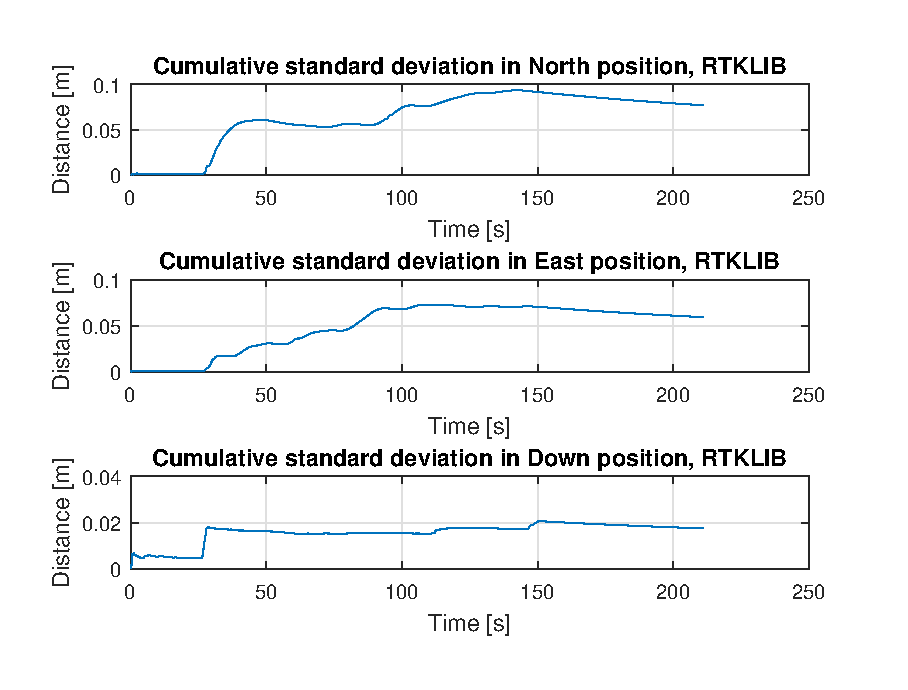
\includegraphics[width=0.7\textwidth]{figs/plots/stdRtklibWalk1.eps}
		\caption{Standard deviation of the difference between rtklib real time and post processed solution}
		\label{figure:stdRTK}
\end{figure}
\begin{figure}[H]
	\centering
		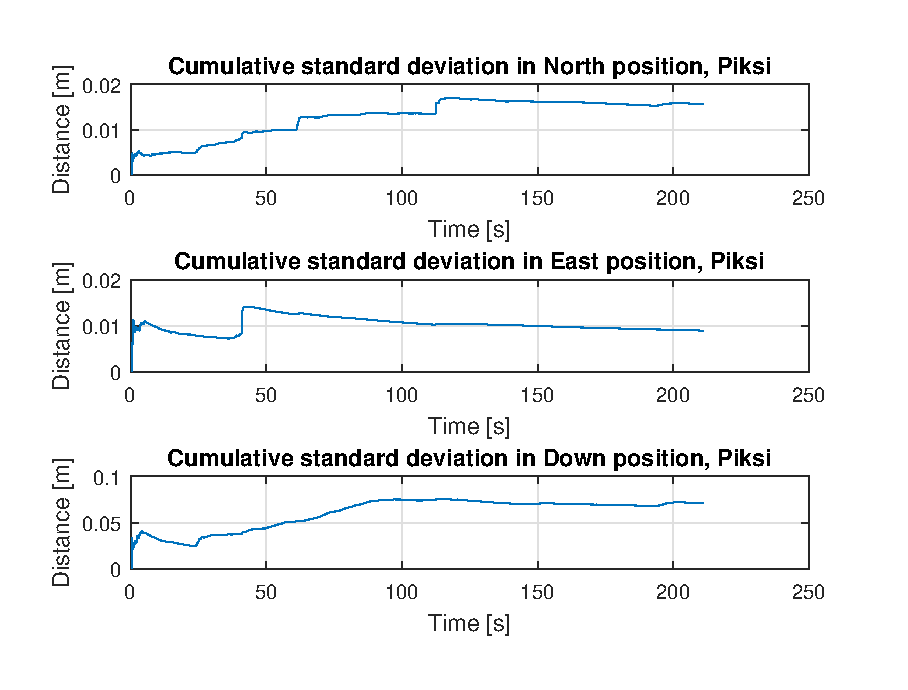
\includegraphics[width=0.7\textwidth]{figs/plots/stdPiksiWalk1.eps}
		\caption{Standard deviation of the difference between piksi real time and rtklib post processed solution}
		\label{figure:stdPiksi}
\end{figure}
Both the Piksi and \gls{rtklib} agrees to the same estimate the North and East velocity, as seen in figure \ref{figure:VelocityWalk1}. However the Down velocity from \gls{rtklib} is more noisy then the Piksi. This behaviour could be introduced because the \gls{uav} was carried around.
\begin{figure}[H]
	\centering
		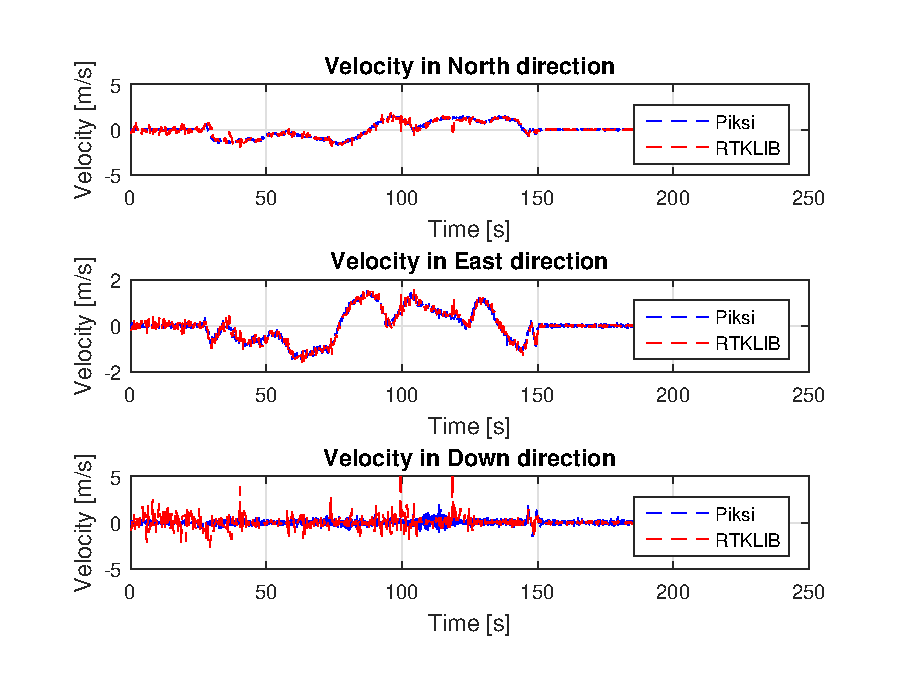
\includegraphics[width=0.7\textwidth]{figs/plots/velocityWalk1.eps}
		\caption{Velocity data from the piksi and rtklib real time solution}
		\label{figure:VelocityWalk1}
\end{figure}
%The problem with the \gls{tow} is shown more clearly in figure \ref{figure:timeRTKwalk1}. The figure display the time difference between each output. The first part is an altered version of the \gls{tow} from rtklib, while the other is the timestamp of the same output given by Dune. The output from rtklib gave only seconds, and not a millisecond value. To correct for this error the \gls{tow} value from rtklib altered to fill the gap between each second. The alteration was done by counting the number of elements with the same \gls{tow} value, and then equally spread them from between the \gls{tow} value to the next \gls{tow} value.
%
%The timestamp given by Dune indicate the delay a output message from rtklib might experience before it's available for consumption. Both the timestamp and \gls{tow} value indicate that rtklib has a mean output of 5 Hz. Here it should be noted that the ublox was configured with a output rate of 10 Hz.
%\begin{figure}[H]
%	\centering
%		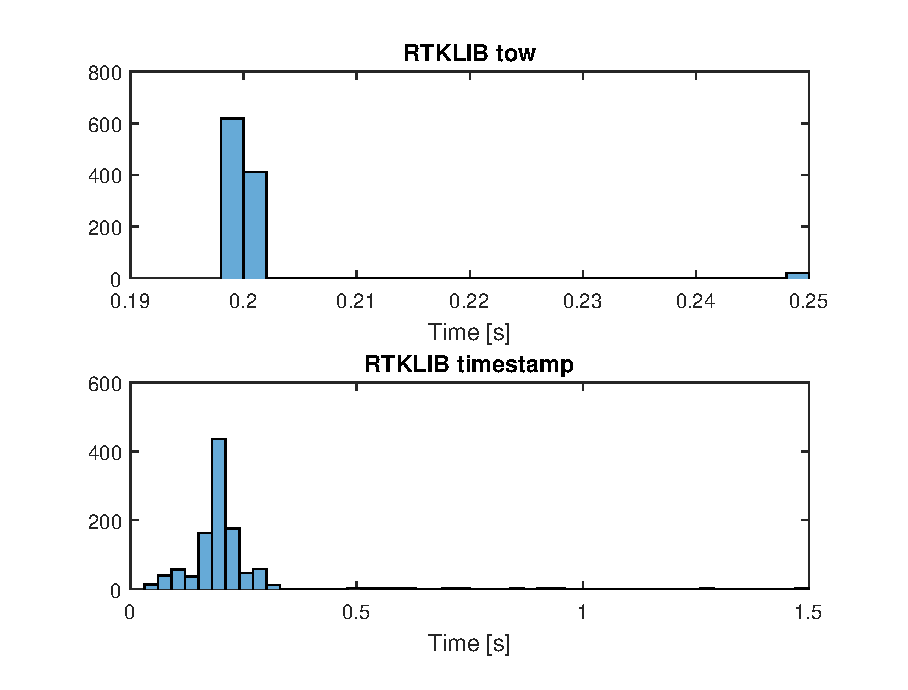
\includegraphics[width=0.7\textwidth]{figs/plots/rtktime.eps}
%		\caption{The time between time samples from rtklib}
%		\label{figure:timeRTKwalk1}
%\end{figure}
%Figure \ref{figure:timePiksiWalk1} shows the time difference between each output sample. The first plot shows the difference between each \gls{tow} value from Piksi, and the other the difference between each time stamp given by Dune. Both plots indicate that Piksi is able to have a output frequency at 10 Hz.
%\begin{figure}[H]
%	\centering
%		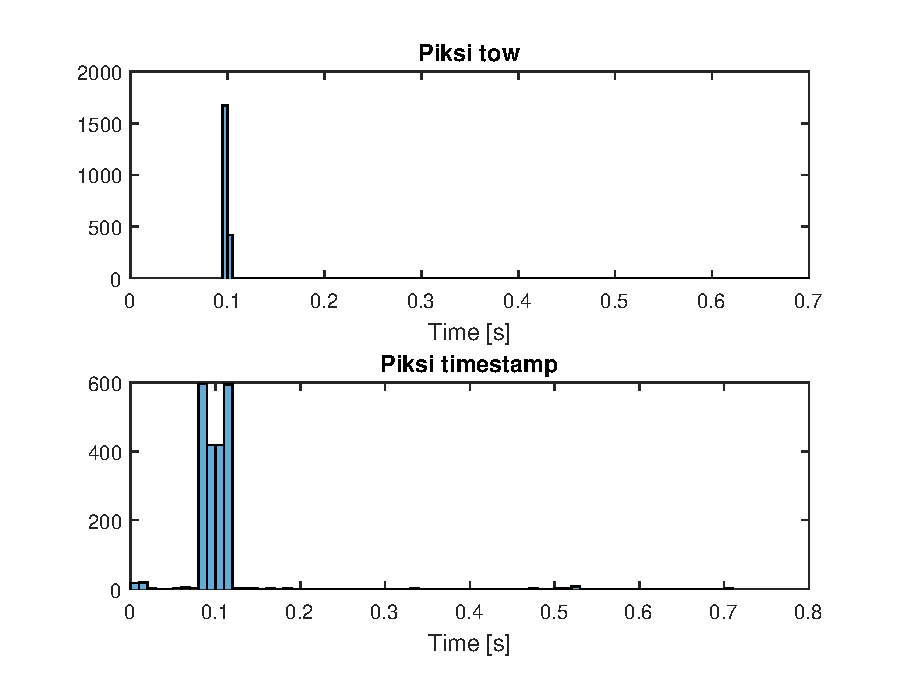
\includegraphics[width=0.7\textwidth]{figs/plots/piksitime.eps}
%		\caption{The time between time samples from rtklib}
%		\label{figure:timePiksiWalk1}
%\end{figure}
The different receiver used in Rtklib and Piksi was not able to track the same satellites at all time. Figure \ref{figure:NumSatWalk1} shows that the Ublox LEA M8T receiver connected to Rtklib managed to track more satellite then the receiver used in Piksi. 
\begin{figure}[H]
	\centering
		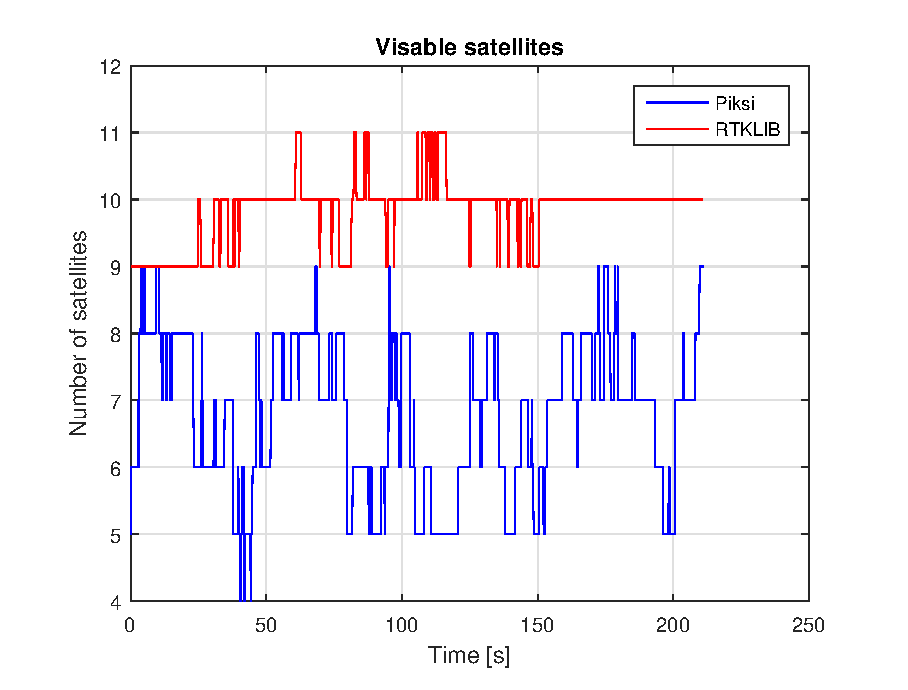
\includegraphics[width=0.7\textwidth]{figs/plots/numSatWalk1.eps}
		\caption{Visable statellite for the piksi and rtklib}
		\label{figure:NumSatWalk1}
\end{figure}
The position estimate of the rover is a relative position in reference to the base station. Due to the fact that the position of the base station is calculated with a single receiver with one frequency, there will be introduced a bias in the position estimate. Figure \ref{figure:enhancedxywalk1} shows the North, East position of the the first walk. The true position is exactly the same, but in the figure the distance is approximately $5-10cm$. The distance from the base station to the estimated start and stop position was calculated to be $3.3553m$ and $3.2914m$ respectfully. The measured distance was approximately $3.3m$. That gives an initial error off $0.02m$. This gives an accuracy level at centimeter level at stationary condition. 
\begin{figure}[H]
	\centering
		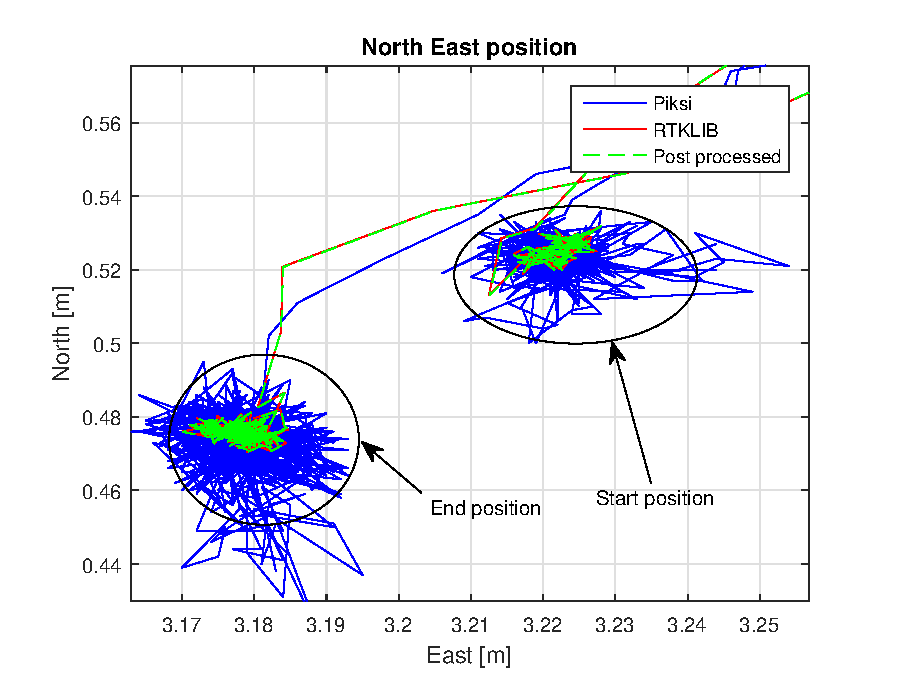
\includegraphics[width=0.7\textwidth]{figs/plots/enhancedxywalk1.eps}
		\caption{Visable statellite for the piksi and rtklib}
		\label{figure:enhancedxywalk1}
\end{figure}
The position estimate from \gls{rtklib} is delayed in comparison to the solution from the Piksi. Figure \ref{figure:DownDelay} shows that both the post processed solution and the real time solution is delay by $0.5$ secounds compared to the Piksi. This could be how \gls{rtklib} resolve the millisecond in \acrfull{tow}, and may not be seen as an extra delay seen from the control systems perspective.
\begin{figure}[H]
	\centering
		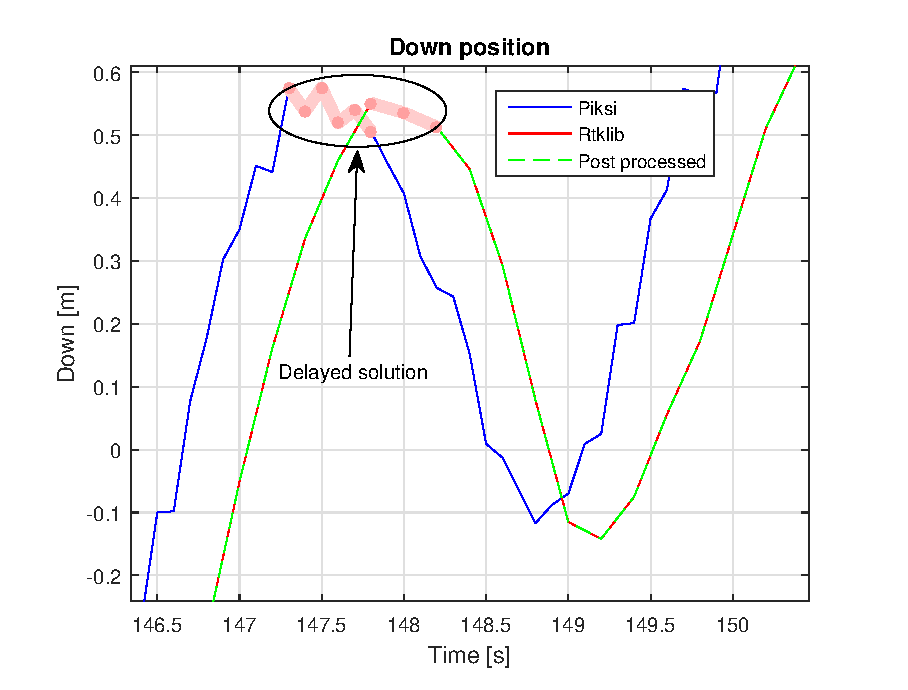
\includegraphics[width=0.7\textwidth]{figs/plots/downDelay.eps}
		\caption{Velocity data from the piksi and rtklib real time solution}
		\label{figure:DownDelay}
\end{figure}
Given that the error given in figure \ref{figure:errorPiksiwalk1} and \ref{figure:errorRTKwalk1} is never has a greater absolute value then $0.2m$ it's possible to assume that the true error will be bellow $1m$ which was given as an evasion criterion in the MSc thesis by \citep{Froelich}, if the \gls{rtk-gps} system has a fixed integer solution.
\subsubsection{Second test}
The second session was perform few minutes after the first, with the same weather condition.
During the second session the Piksi lost its fixed integer solution, while Rtklib managed to keep its fixed integer solution as seen in figure \ref{figure:xyWalk2} and \ref{figure:downWalk2}.

\begin{figure}[H]
\begin{subfigure}[H]{1\textwidth}
	\centering
		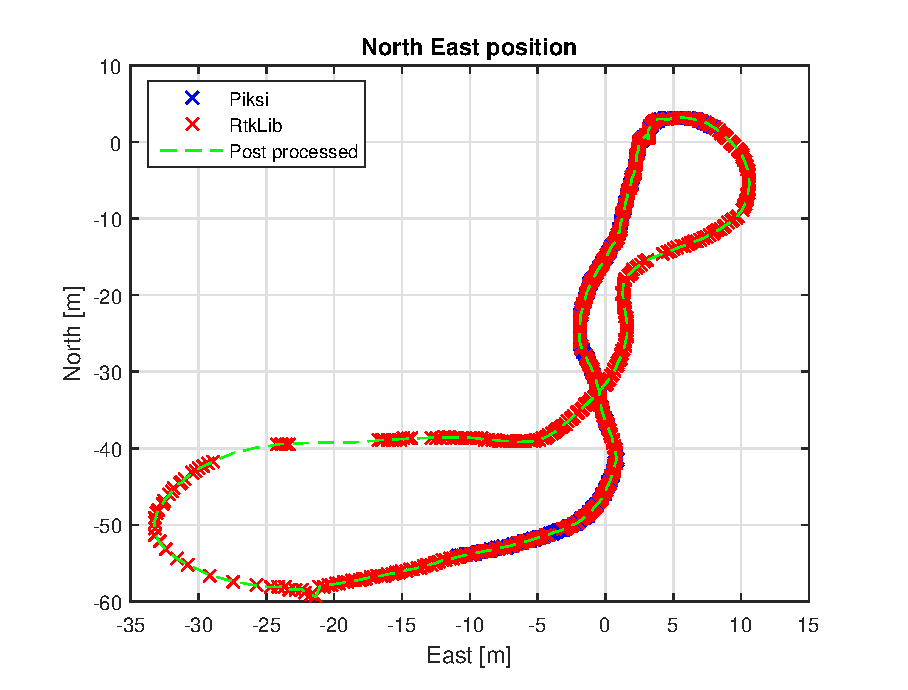
\includegraphics[width=0.7\textwidth]{figs/plots/xywalk2.eps}
		\caption{Visable statellite for the piksi and rtklib}
		\label{figure:xyWalk2}
\end{subfigure}
%\end{figure}
%\begin{figure}[H]
\begin{subfigure}[H]{1\textwidth}
	\centering
		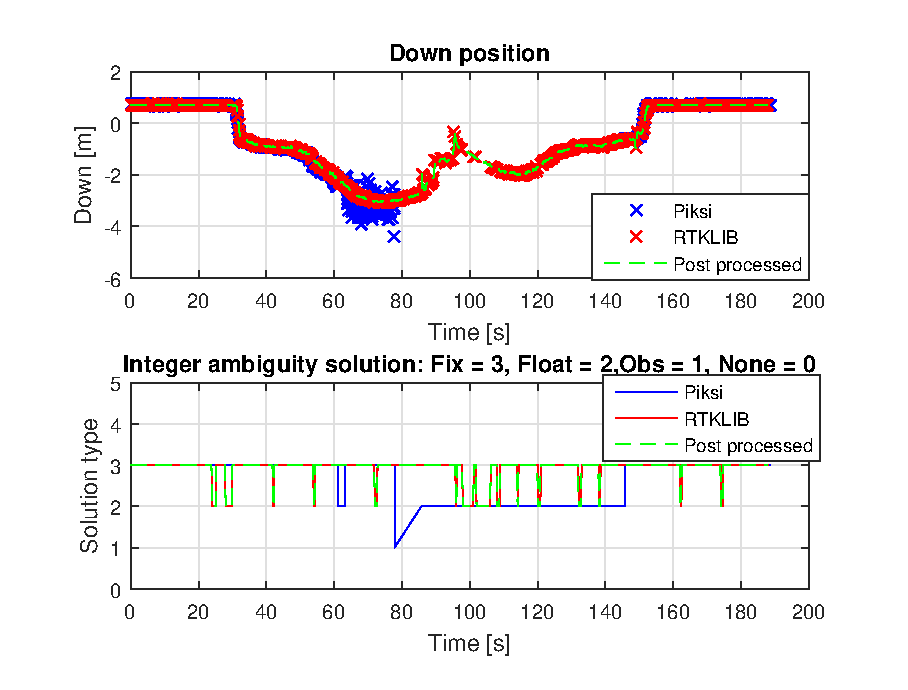
\includegraphics[width=0.7\textwidth]{figs/plots/downWalk2.eps}
		\caption{Visable statellite for the piksi and rtklib}
		\label{figure:downWalk2}
\end{subfigure}

\end{figure}
The reason for why the Piksi lost its fixed solution might be because it lost track of several satellite, as seen in figure \ref{figure:numSatWalk2}. Since both receive share the same antenna it can be concluded that the satellite tracing performance in the Ublox is superior to the Piksi.  Even when the Piksi managed to regain track of the satellite it lost, it took 60 seconds before it regain a fixed integer solution. 
\begin{figure}[H]
	\centering
		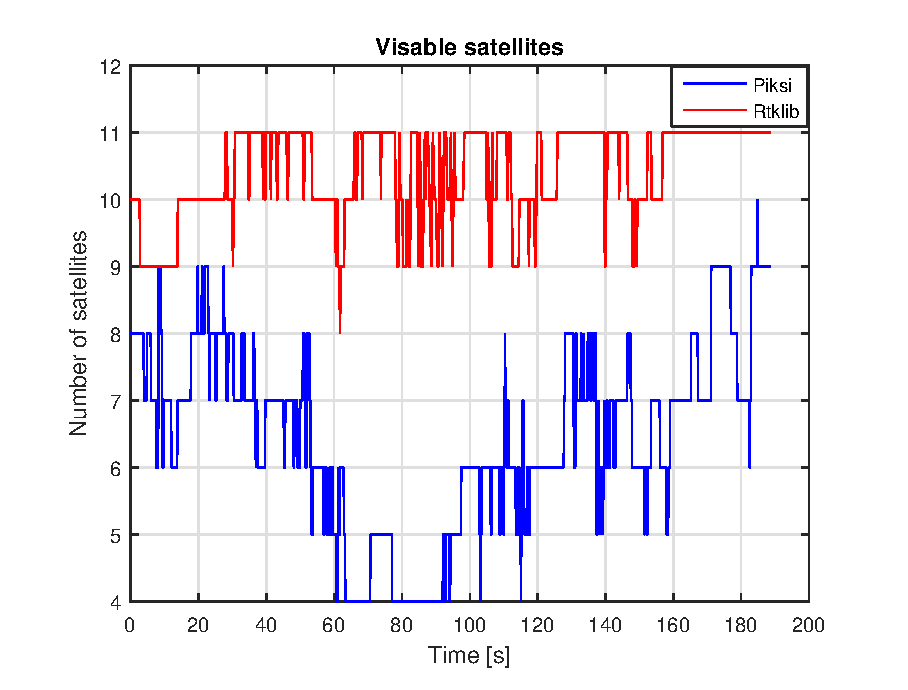
\includegraphics[width=0.7\textwidth]{figs/plots/numSatWalk2.eps}
		\caption{Visable statellite for the piksi and rtklib}
		\label{figure:numSatWalk2}
\end{figure}
\subsection{In-flight test}
A flight test with the \gls{uav} was performed at Udduvoll. Because of bad weather the were only performed one flight, and before the flight started only the Rtklib had a fixed solution. That is why in this part only performance from the Rtklib is considered, as a navigation system must have a fixed solution before the automatic net landing system can start.

During the flight test the integer ambiguity solution were more float then fixed as seen in figure \ref{figure:DownFlight} and \ref{figure:NorthEastFlight}, which affected the measurement. The same behaviour will be seen during the landing, however if the float solution is accurate enough the system should be able to perform a automatic landing.
\begin{figure}[H]
	\centering
		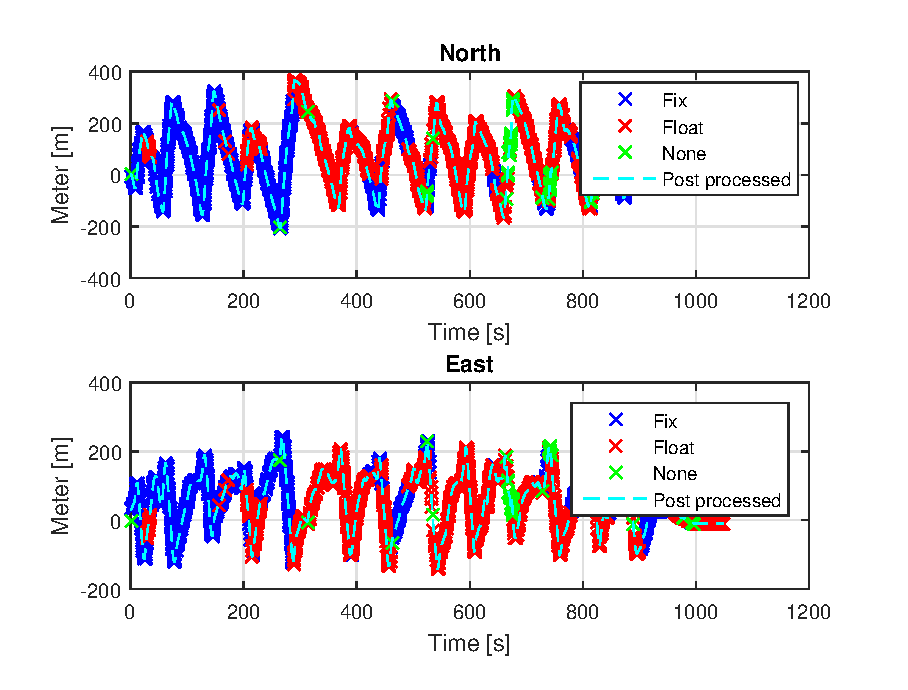
\includegraphics[width=0.7\textwidth]{figs/plots/northEastFlight.eps}
		\caption{Velocity data from the piksi and rtklib real time solution}
		\label{figure:NorthEastFlight}
\end{figure}
\begin{figure}[H]
	\centering
		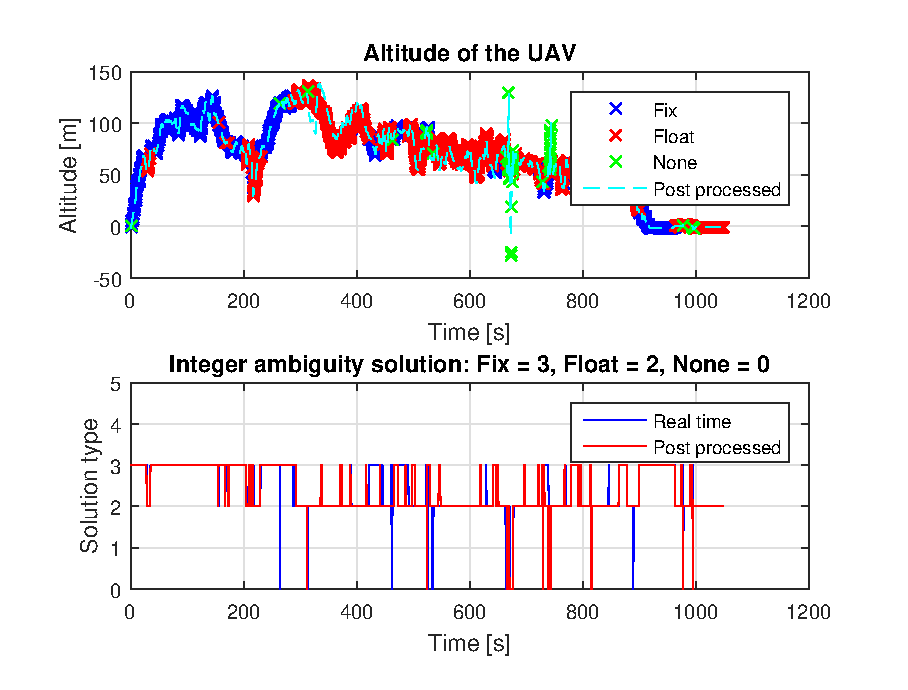
\includegraphics[width=0.7\textwidth]{figs/plots/AltitudeFlight.eps}
		\caption{Velocity data from the piksi and rtklib real time solution}
		\label{figure:DownFlight}
\end{figure}
The main reason for the lost fixed solution is because of the number of valid satellite the receiver can track experience large variation, as seen i figure \ref{figure:numSatFlight}. A problem that was experienced during the flight is that large roll and pitch angel of the \gls{uav} blocks the antennas view of different satellites. That is a problem that can be solved by setting restriction on the dynamical behaviour of the \gls{uav} especially before and during landing.
\begin{figure}[H]
	\centering
		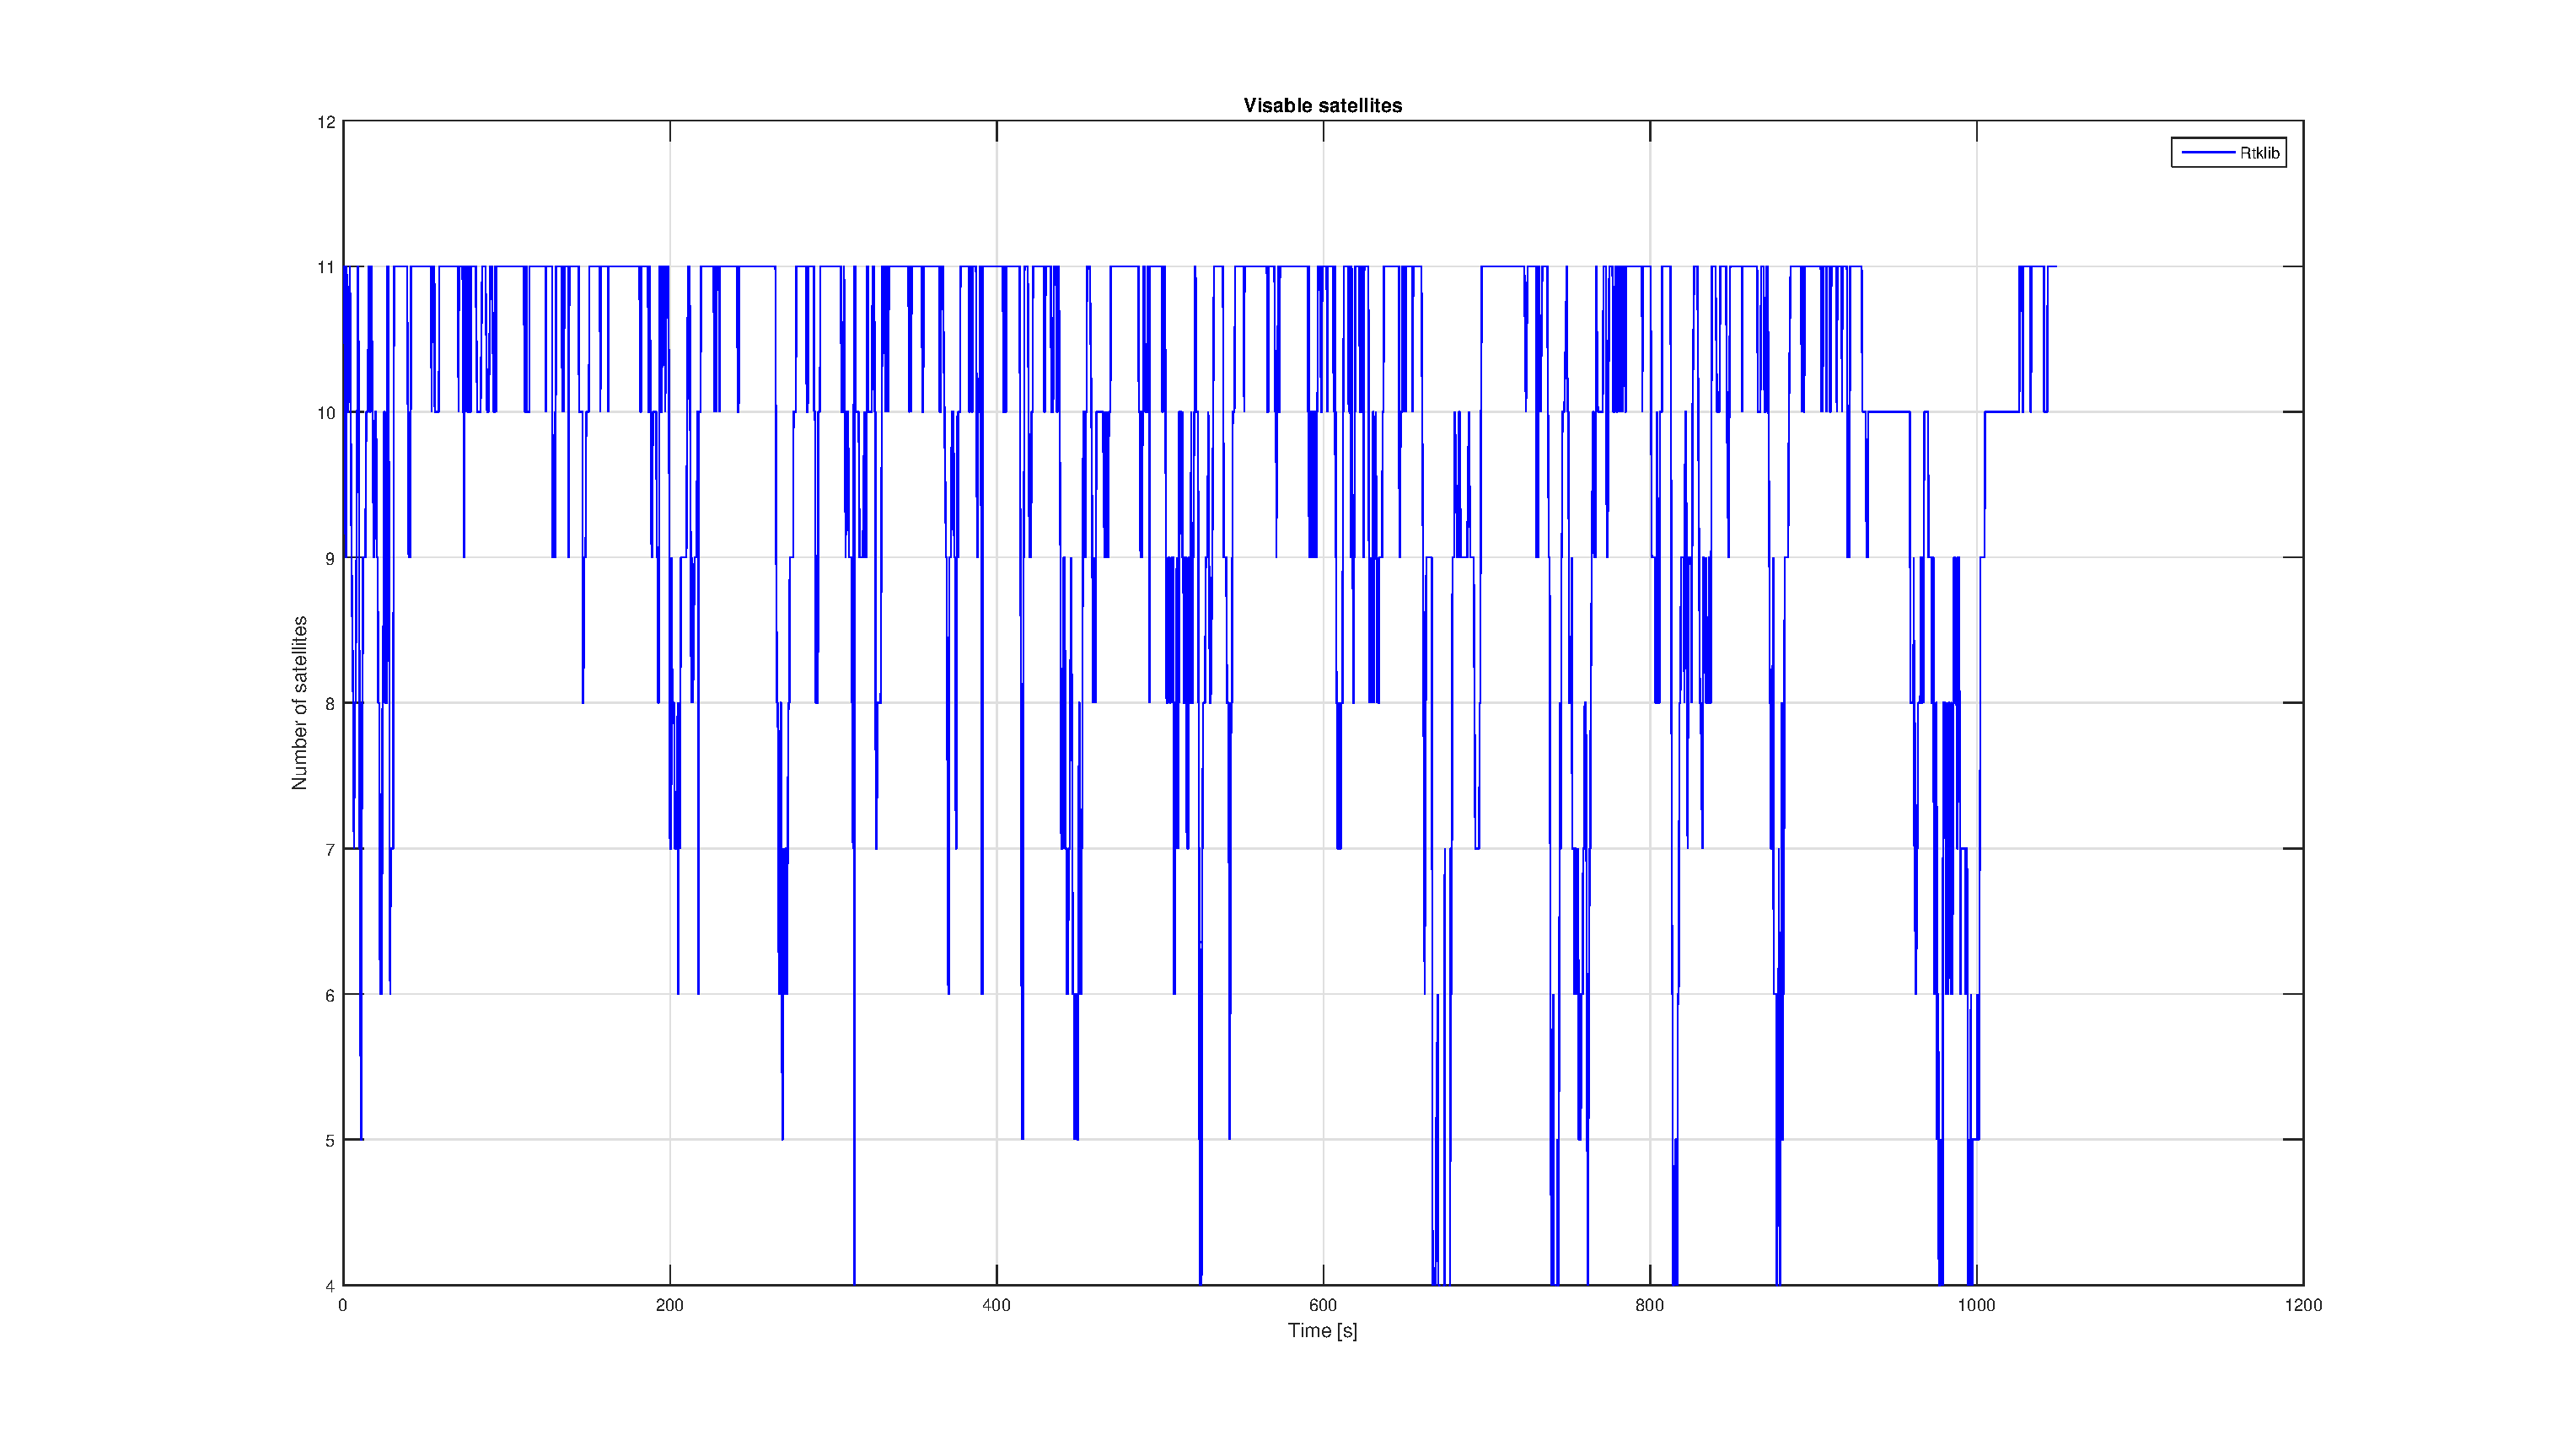
\includegraphics[width=0.7\textwidth]{figs/plots/numSatFlight.eps}
		\caption{Velocity data from the piksi and rtklib real time solution}
		\label{figure:numSatFlight}
\end{figure}
%\begin{figure}[H]
%	\centering
%		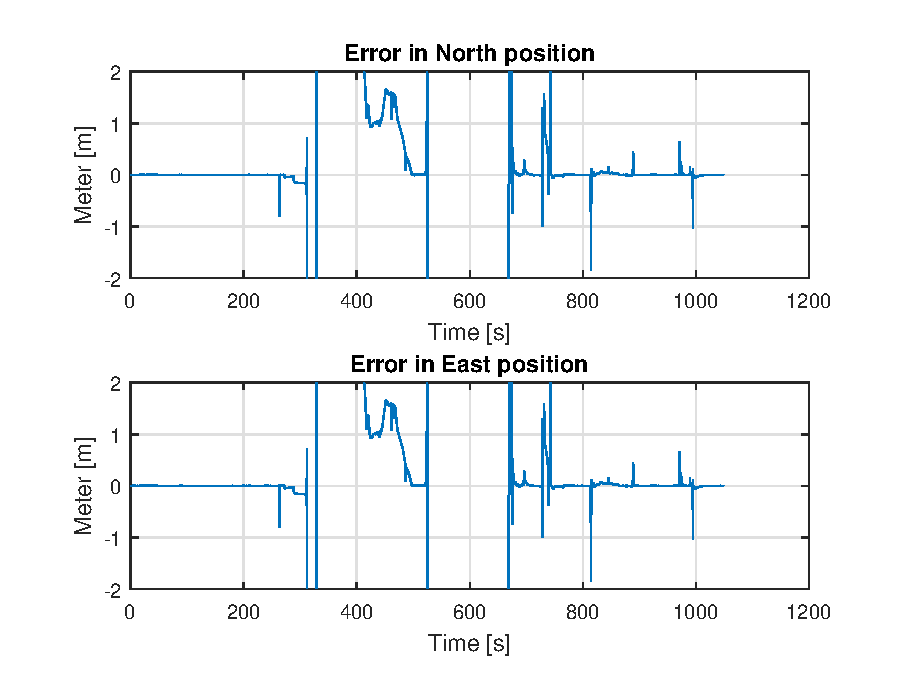
\includegraphics[width=0.7\textwidth]{figs/plots/errorNorthEastFlight.eps}
%		\caption{Velocity data from the piksi and rtklib real time solution}
%		\label{figure:errorNorthEastFlight}
%\end{figure}
%\begin{figure}[H]
%	\centering
%		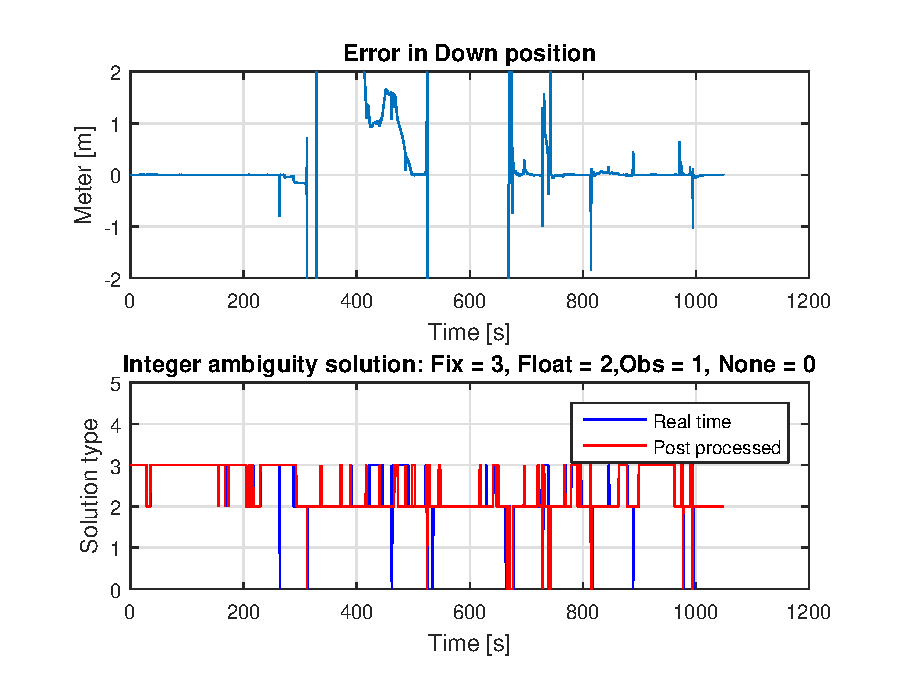
\includegraphics[width=0.7\textwidth]{figs/plots/errorDownFlight.eps}
%		\caption{Velocity data from the piksi and rtklib real time solution}
%		\label{figure:errorDownFlight}
%\end{figure}
\subsubsection{Landing}
As expected the \gls{rtk-gps} system had problem with keeping it's fixed integer solution. The \gls{rtk-gps} position estimate of the landing path is shown in figure \ref{figure:landingPath}. The system kept changing between float and fixed solution during the landing phase. Figure \ref{figure:landingNorthEastFlight} shown the North East position during the landing with the type of solution. The Down position as well as the integer ambiguity solution is for the landing phase is seen in \ref{figure:landingDownFlight}. The \gls{rtk-gps} system was unable to maintain a fixed solution, however it did maintain a float solution. Further test with a control system is required in order to test if also the float solution is accurate enough to perform a automatic net landing.
\begin{figure}[H]
	\centering
		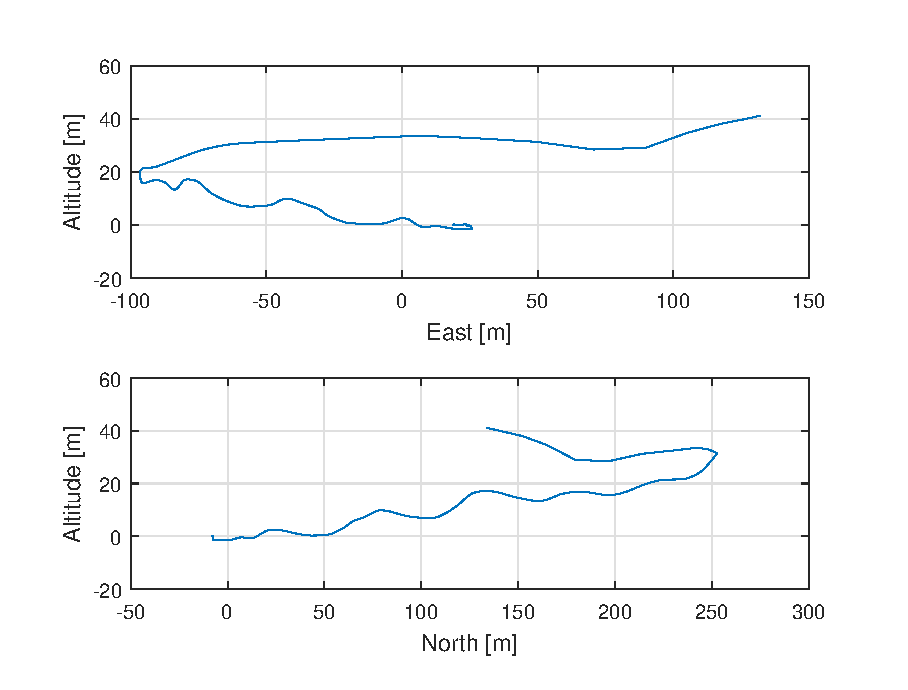
\includegraphics[width=0.7\textwidth]{figs/plots/landingPath.eps}
		\caption{Velocity data from the piksi and rtklib real time solution}
		\label{figure:landingPath}
\end{figure}
\begin{figure}[H]
	\centering
		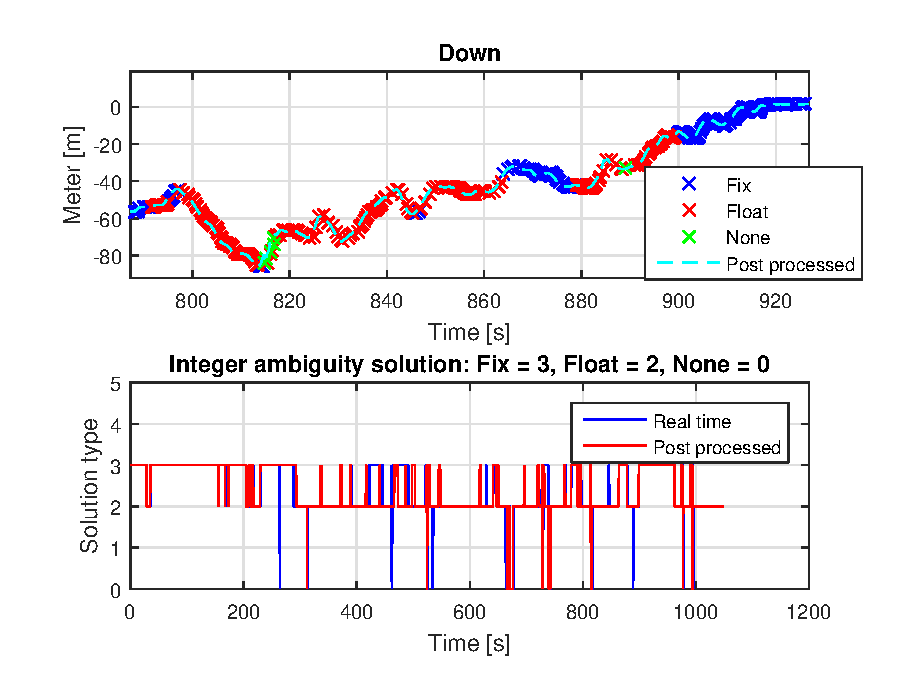
\includegraphics[width=0.7\textwidth]{figs/plots/landingDownFlight.eps}
		\caption{Velocity data from the piksi and rtklib real time solution}
		\label{figure:landingDownFlight}
\end{figure}

From the error plot seen in figure \ref{figure:landingErrorNorthEastDownFlight} it appear that to be able to estimate it's own position with an error bellow 1 meter most of the time. However this is compared to the post processed estimate, which also will diverge from the true value since it is based on the same raw data as the real time solution.

\begin{figure}[H]
	\centering
		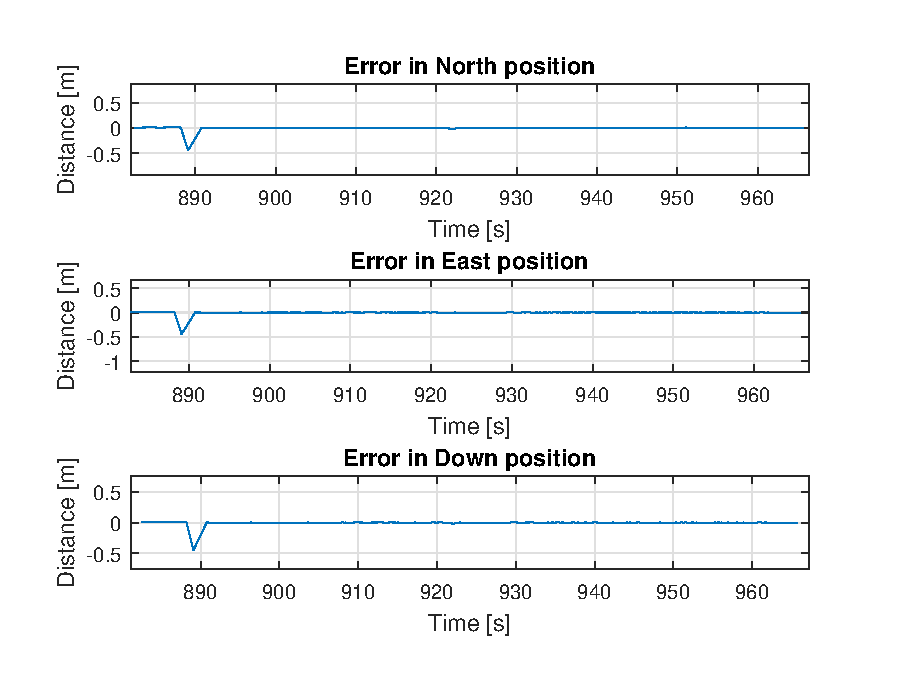
\includegraphics[width=0.7\textwidth]{figs/plots/landingErrorNorthEastDownFlight.eps}
		\caption{Velocity data from the piksi and rtklib real time solution}
		\label{figure:landingErrorNorthEastDownFlight}
\end{figure}
The landing velocity seen in figure \ref{figure:landingVelocity} confirms the precision in the estimate that was seen in the first test. However the altitude velocity is less noisy, and can be used in a control system.
\begin{figure}[H]
	\centering
		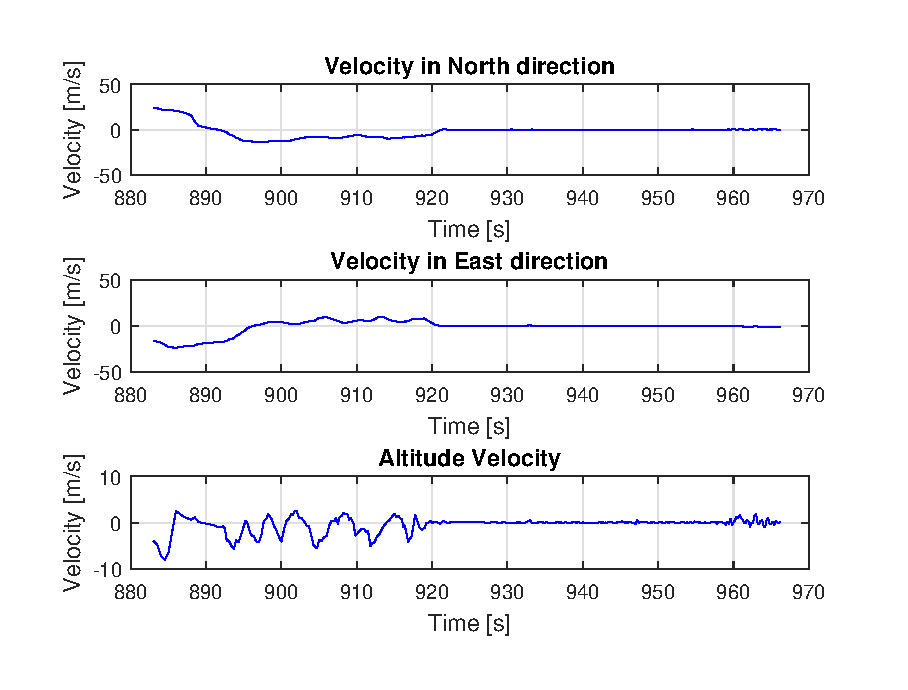
\includegraphics[width=0.7\textwidth]{figs/plots/landingVelocity.eps}
		\caption{Velocity data from the piksi and rtklib real time solution}
		\label{figure:landingVelocity}
\end{figure}
\cleardoublepage